\chapter{Uvrščanje}

Uvrščanje v skupine ali klasifikacija predpostavlja, da je za dani nabor primerov podan tudi razred. Novice na primer lahko pripadajo razredu šport, poslovne novice, razvedrilo. Uporabniki telekomunikacijskih storitev so lahko zvesti ali pa po določenem času zbežijo k drugemu ponudniku \angl{churn}. Spletna stran je lahko dobro ali slabo obiskana. Izdelek v prodajalni je lahko prodajan z dobičkom ali pa izgubo.

V vseh zgornjih ali pa podobnih primerih bi želeli primere uvrstiti v razrede na podlagi njihovega atributnega opisa. Pri predmetih s področja umetne inteligence in inteligentnih sistemov ste že spoznali nekaj tehnik strojnega učenja, ki so temu primerne, tu pa bi želeli dodatno opisati (ali pa vsaj ponoviti) nekaj pristopov, ki so pomembni za sisteme poslovne inteligence, vključno z:

\begin{itemize}
\item predobdelavo podatkov, na primer izbor najbolj informativnih atributov,
\item izbor tehnike za uvrščanje v skupine oziroma določitev parametrov izbrane metode,
\item vrednotenje uspešnosti napovedovanja razredov,
\item razlaga uvrstitve oziroma predlagane odločitve.
\end{itemize}

\section{Ocenjevanje pomembnosti atributov\label{c-attribute-scoring}}

Pri prav vseh praktičnih problemih uvrščanja v skupine nas zelo zanimajo atributi, ki so kar najbolj povezani z znanimi uvrstitvami primerov oziroma, kot bi temu rekli v strojnem učenju, z razredi primerov. Razkritje takih atributov nam lahko dosti pove o problemu, ki ga raziskujemo, odkrije, katere lastnosti opazovanih objektov moramo spremljati še v prihodnje oziroma so tiste, ki igrajo pomembno vlogo pri računalniški podpori odločanja. Velika večina tehnik ocenjevanj pomembnosti atributov obravnava en sam atribut ločeno od ostalih, to je, zanemari kakršnekoli medsebojne povezanosti atributov. Peščica tehnik, med katerimi bomo tu omenili eno samo, najbolj znano, pa zna razkriti pomembnost atributa tudi z ozirom na kontekst, to je, skladno z vrednostmi ostalih atributov.

Začnimo pri tehnikah, ki atribute obravnavajo vsakega zase in kontekst ostalih atributov zanemarijo. Za začetek poglejmo množico trikotnikov in kvadratov s slike~\ref{f-squares-triangles}. Želeli bi oceniti, kako dobro lahko na podlagi barve lika napovemo njegovo obliko. 

\begin{figure}[htbp]
\begin{center}
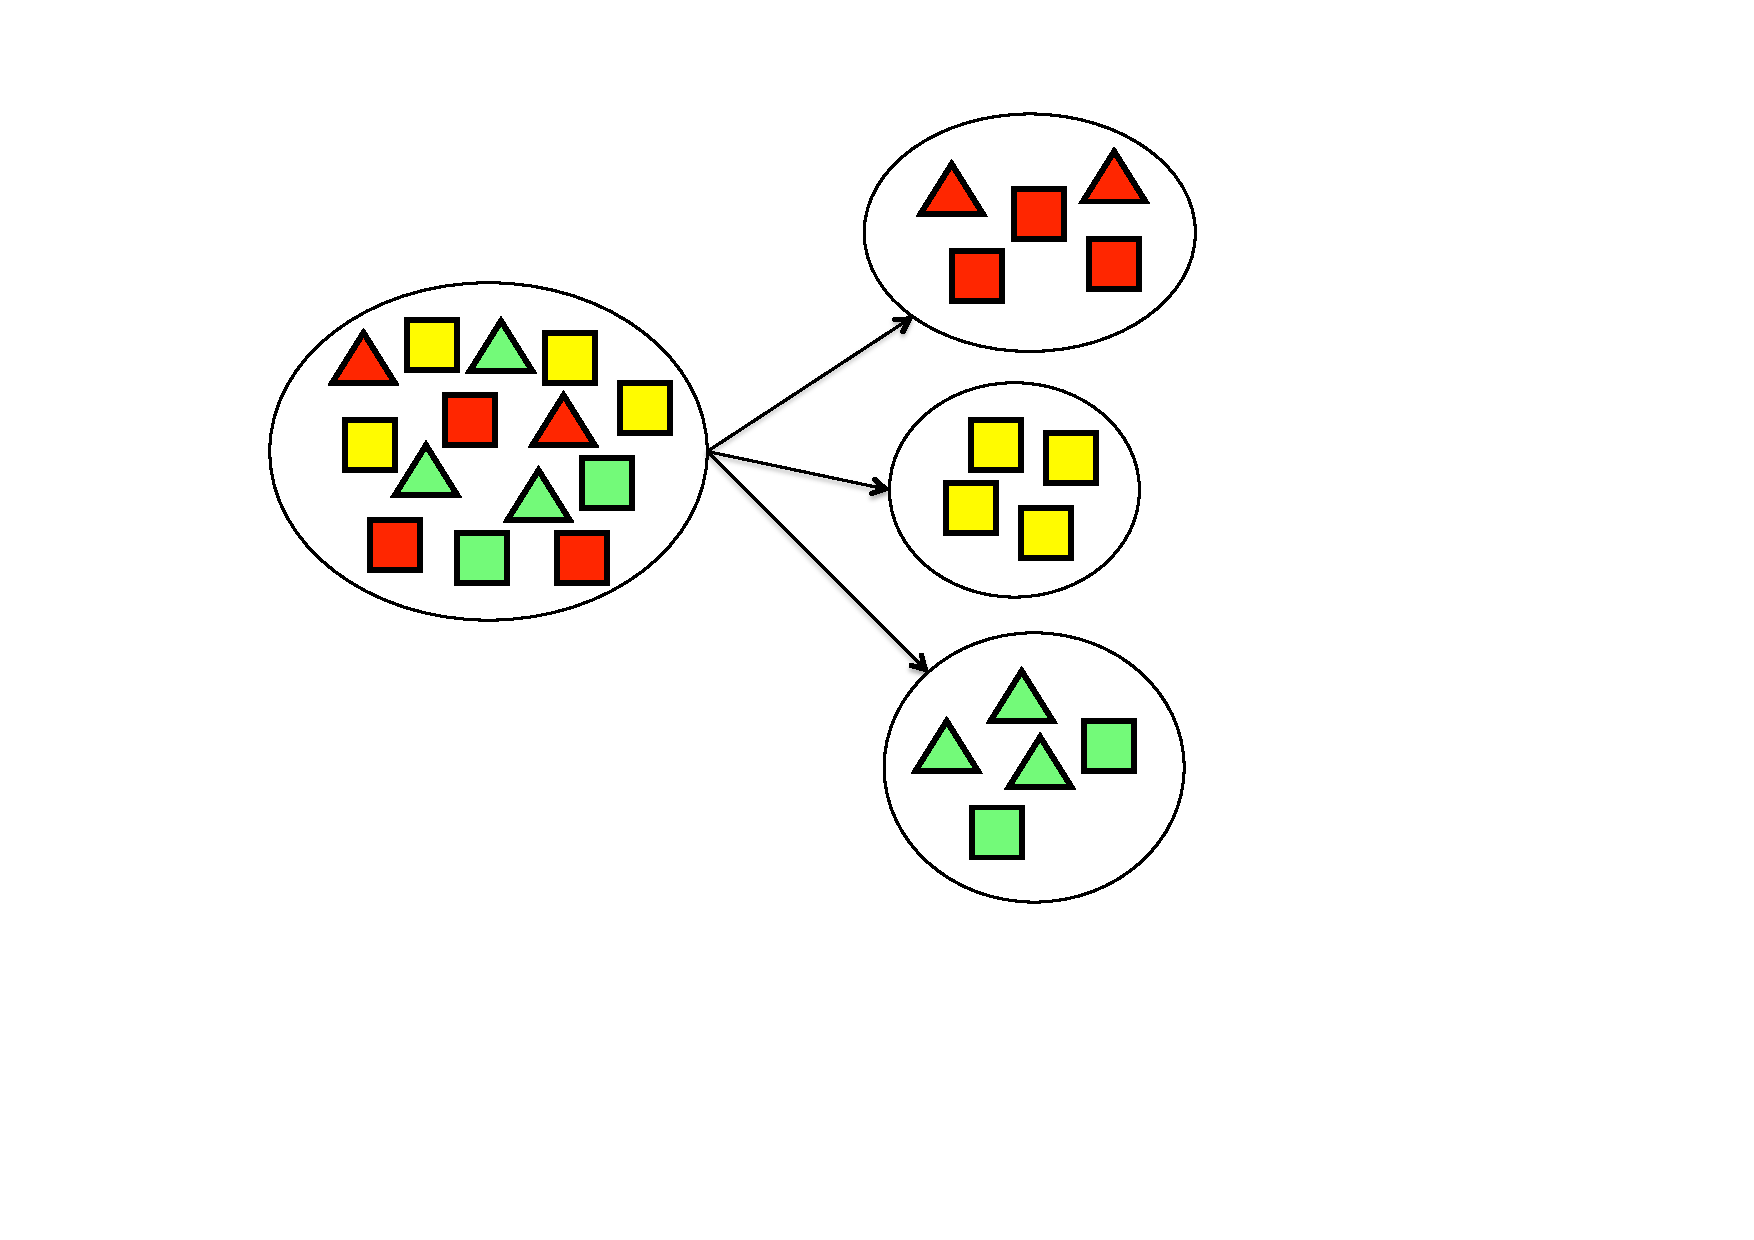
\includegraphics[width=7cm]{slike/squares-triangles.pdf}
\caption{Množica različno obarvanih kvadratov in trikotnikov (levo) in ista množica razdeljena na tri podmnožice glede na barvo likov. Vseh likov skupaj je $N=14$.}
\label{f-squares-triangles}
\end{center}
\end{figure}

\subsection{Informacijski prispevek}

Če bi bila povezanost med barvami in oblikami likov popolna, bi bile v posameznih podmnožicah na desni strani slike~\ref{f-squares-triangles} vsi liki enakih oblik. Pa niso. Pravimo, da množice niso čiste. Podmnožica rumenih likov je čista, čistočo ostalih pa bi radi zmerili. Obliko likov, naš razred, obravnavajmo kot naključno spremenljivko $C$, njene vrednosti pa označimo z $c_i$. Naša spremenljivka ima dve različni vrednosti, ``trikotnik'' in ``kvadrat''. Ocenimo še verjetnosti, da med liki iz naše celotne množice likov ($N=14$) izberemo, na primer, trikotnik. Za oceno uporabimo kar relativno frekvenco:
%
$$ P_{\triangle}={N_{\triangle} \over N} = 5/14 = 0.357 $$
%
Podobno izračunamo, da je $P_{\Box}= 0.643$. Nečistočo naše množice likov lahko ocenimo z entropijo $H$ diskretne naključne spremenljive $C$, ki je, izmerjena v bitih:
%
$$ H(C) = \sum_{i=1}^n {p(c_i)\,I(c_i)} = -\sum_{i=1}^n {p(c_i) \log_2 p(c_i)} $$
%
oziroma za naš primer:
$$ H(C) = - 0.357 \times log_2 0.357 - 0.643 \times log_2 0.643 = 0.940 $$

Ravno tako, kot za osnovno množico, lahko ocenimo nečistočo podmnožic, ki jih dobimo, ko smo like razdelili glede na njihovo barvo. Tako dobimo:
%
$$ H(C|{\rm color=red}) = -\plogp{3}{5}-\plogp{2}{5}=0.971 $$
$$ H(C|{\rm color=yellow}) = -\plogp{4}{4}-\plogp{0}{4}=0.0 $$
$$ H(C|{\rm color=green}) = -\plogp{2}{5}-\plogp{3}{5}=0.971 $$

Oceniti moramo še verjetnost, da lik pripada eni od podmnožic. Z drugimi besedami, kakšna je verjetnost, da bo naključno izbran lik iz naše osnovne množice na primer rdeč. Enostavno, 
%
$$ P_{\rm red}={N_{\rm red}\over N} = {5\over 14}=0.357$$
%
Podobno ocenimo še $P_{\rm yellow}=0.286$ in $P_{\rm green}=0.357$. Pričakovana nečistoča podmnožic, ko našo množico likov razdelimo skladno z njihovo barvno, ocenimo kot vsoto nečistoč podmnožic, ki jo utežimo z verjetnostjo, da bo lik pripadal določeni množici. Dobljeni uteženi vsoti pravimo residualna entropija:
%
$$ H_{res}=H(C|X)=\sum_{_i} p(x_i) H(C|x_i)  $$
%
in za naš primer znaša:
$$ H_{res} = 0.357 \times 0.971 + 0.0 \times 0.971 + 0.357 \times 0.971 = 0.694 $$

Pričakovana entropija, ko smo like razdelili po barvi, je torej manjša od entropije osnovne množico. Njuni razliki pravimo informacijski prispevek \angl{information gain} in z njim ocenimo, koliko informacije nam prispeva poznavanje vrednosti posameznega atributa:
$$ {\rm IG}(X) = H(C) - H(C|X) = 0.940 - 0.694 = 0.246 $$

\subsection{Relativni informacijski prispevek}

Pri atributih, ki imajo veliko zalogo vrednosti, se nam prav lahko zgodi, da nam ti primere iz osnovne množice razdelijo v zelo majhne podmnožice, morda celo take s po enim samim elementom. Entropija oziroma nečistoča slednjih je nič, a takih podmnožic si vsekakor ne želimo. Pravzaprav lahko informacijski prispevek favorizira atribute z veliko zalogo vrednosti. To ``prednost'' lahko uravnotežimo s tem, da se vprašamo, koliko informacije potrebujemo, da zvemo vrednost posameznega atributa. V našem primeru imamo med štirinajstimi liki pet rdečih, štiri rumene in pet zelenih, zato:
$$ H(X)=-\plogp{5}{14}-\plogp{4}{14}-\plogp{5}{14}=1.58 $$
%
Mero, kjer vrednost zgornjega izraza uporabimo za uravnoteženje informacijskega prispevka, imenujemo relativni informacijski prispevek \angl{information gain ratio}:
%
$$ {\rm IGR}(X) = {{\rm IG}(X)\over H(X)} $$
V našem primeru je relativni informacijski prispevek barve likov enak $0.246/1.58=0.156$.

Predlagano uravnoteženje ni edini način, da izenačimo ocene za atribute, ki imajo (zelo) različno število vrednosti. Morda bolj naravna, a računsko zahtevnejša je tehnika, ki uporablja permutacijski test in jo omenjamo v nadaljevanju.

\subsection{Mera nečistoče po Giniju}

Prikladna mera nečistoče je tudi ginijev indeks:
$$ {\rm Gini}(C)=\sum_{i}p(C=c_i)\times (1-p(C=C_i)) = 1 - \sum_i [p(C=c_i)]^2 $$
Ta ocena enaka nič za čiste množice, torej množice, kjer vsi primeri pripadajo istemu razredu, in višje vrednosti pri množicah primerov, ki pripadajo različnim razredom. Nečistoča po Giniju pove, kako pogosto bi bil za naključno izbran primer napačno napovedan razred, ki bi ga uteženo naključno napovedali iz dane porazdelitve razredne spremenljivke.

\subsection{ReliefF}

Uvedbo mere imenovane ReliefF motivirajmo na primeru s tabele~\ref{t-xor-boat}. Primer povzema okoliščine in rezultat odločitve prijatelja jadralca, ki razmišlja, ali naj gre na morje glede na družbo, barko in jakost vetra. Prav vse mere za ocenjevanje atributov, ki smo jih omenjali zgoraj, ocenijo, da na podlagi atributov ``boat'' in ``wind'' ne moremo ničesar povedati o razredu. Vrednost vseh zgornji mer za ta dva atributa je namreč nič.

\begin{table}[htbp]
\caption{Primer podatkov s tremi atributi in razredom.}
\label{t-xor-boat}
\begin{center}
\begin{tabular}{llll}
\toprule
\multicolumn{3}{c}{Atributi} & Razred \\ \cmidrule(r){1-3} \cmidrule(r){4-4}
company & boat & wind & sailing \\
\midrule
yes & small & mild & no \\
no & small & strong & yes \\
yes & big & strong & yes \\
no & big & strong & no \\
yes & small & strong & no \\
no & small & mild & yes \\
yes & big & mild & yes \\
no & big & strong & no \\
\bottomrule
\end{tabular}
\end{center}
\end{table}

Pa sta omenjena atributa res nepomembna? Ali res na podlagi njih ne moremo prav nič reči o razredu? 

Kaj pa, če za upravljanje večje barke potrebuje nekaj prijateljev, manjšo pa bo znal v kakršnihkoli pogojih obvladati sam? Zares, podatki govorijo prav o taki povezanosti med atributoma. Vsak atribut sam zase ne pove ničesar o razredu, a skupaj, v kombinaciji, podata atributa popolno informacijo. Mere, ki obravnavajo vsak atribut posebej, brez konteksta, nam uporabnost atributov, ki so na nek način povezani z ostalimi atributi in z njimi v kombinaciji razkrivajo razred, ne bodo odkrile.

Mero, ki razkrije uporabnost atributov tudi v takih primerih kot je ta s slike~\ref{t-xor-boat}, sta prva predlagala Kira in Rendell~\cite{} in jo poimenovala Relief. Za vsak primer $X$ Relief poišče njemu najbližji primer $X_{hit}$ istega razreda (bližnji zadetek) in najbližji primer $X_{miss}$ različnega razreda (bližnji pogrešek). Bližino primerov ocenimo na podlagi vseh atributnih vrednosti s kakšno od mer, ki smo jih spoznali v prejšnjih poglavjih. Atribut, ki je koristen za napovedovanje razreda, bi morali imeti v primerih $X$ in $X_{hit}$ podobne vrednosti, v primerih $X$ in $X_{miss}$ pa čimbolj različne vrednosti. S tem smo intuitivno že orisali algoritem Relief, ki se sprehodi po vseh primerih in oceno atributov, ki je na pričetku enaka 0, popravi z mero različnosti za vrednosti atributa tako, da pri primerjanju z $X_{miss}$ to mero prišteje, pri primerjanju z $X_{hit}$ pa odšteje. V splošnem lahko zapišemo:

\begin{eqnarray}
{\rm Relief(X)} & = & P({\rm razlicna\ vrednost\ atributa}\ |\ {\rm bliznji\  pogresek}) − \nonumber \\
& & P({\rm razlicna\ vrednost\ atributa}\ |\ {\rm bliznji\ zadetek})
\end{eqnarray}

Kononenko~\cite{} je Relief razširil tako, da je ta upoštevala več najbližjih sosedov in jo prilagodil različnim vrstam atributov. Namesto po vseh primerih, kar zna biti časovno zahtevno za večje množice, se njegova razširitev sprehodi preko naključno izbranih primerov ter tem namesto enega samega soseda poišče nekaj najbližjih primerov. Mera, ki jo avtor poimenoval ReliefF, je postala danes najbolj znana kontekstno-odvisna cenilka pomembnosti atributov.

Pri naši množici primerov s tabele~\ref{t-xor-boat} Relief ne zgreši, ampak pravilno ovrednoti informativna atributa in jim pripiše pozitivno oceno. Nista pa ne Relief ne ReliefF brez pomankljivosti. Kontekst namreč ocenita z izborom najbližjih sosedov. Če je atributov mnogo, na primer, več sto ali tisoč, se vloga so-dejavnih atributov porazgubi in tudi ta mera izgubi na moči in ne prepozna pomembnih atributov, katerih vloga bi bila odvisna od konteksta.

\subsection{Permutacijski test}

Pri merah, kot je večina zgornjih, včasih le težko ločimo med informativnimi in neinformativnimi atributi. Pri kakšni vrednosti mere postaviti mejo? Še težje se odločimo, če uporabljamo različne mere, kjer bi za vsako morali poznati njene statistične lastnosti. Je vrednost ocene ReliefF, ki je enaka $0.42$, dovolj visoka, da razglasimo, da je atribut informativen. Kaj pa $0.12$? Pa $0.06$? Dobro bi bilo vedeti, ali so vrednosti teh ocen pozitivne zaradi resničnih zakonitosti v podatkih ali pa smo jih dobili po naključju. Še posebej bodo ta vprašanja zanimiva za probleme, kjer je primerov malo, atributov pa veliko. 

Ocene informativnosti atributov, ki jih dobimo za vsakega od atributov, lahko primerjamo z njihovimi ničelnimi porazdelitvami, ki bi jih dobili, če bi informativnosti ocenjevali na naključno pridobljenih podatkih. Za slednje bo za nekontekstne mere dovolj premešati vrednosti razredne spremenljivke, za ReliefF ali podobne pa bo potrebno premešati celotno tabelo podatkov tako, da bomo premešali vrednosti v vsaki koloni (po atributu, torej) in na ta način ``pokvarili'' morebitni kontekst.

Za naključno premešanje razredne spremenljivke nam lahko služi spodnji razred v Pythonu. Ta si ob inicializaciji zapomni tudi izvorno uvrstitev razredov, ki jo lahko uporabi za vzpostavitev začetnega stanja. Razred je implementiran tako, da podatke ne podvaja, zapomni pa si samo vektor razredov.

\begin{python}
import random

class PermuteClass:
    """Permute the class column of the data, can also restore to original."""
    def __init__(self, data):
        self.c_vals_backup = [d.get_class() for d in data]
        self.c_vals = [d.getclass() for d in data]
    def __call__(self, data):
        random.shuffle(self.c_vals)
        for d, c in izip(data, self.c_vals):
            d.set_class(c)
    def restore(self, data):
        for d, c in izip(data, self.c_vals_backup):
            d.set_class(c)
\end{python}

Razred za premešanje vrednosti razredne spremenljivke uporablja spodnja koda, ki za vsak atribut v podatkih zgradi ničelno porazdelitev atributnih ocen.

\begin{python}
import Orange.data

epochs = 1000
alpha = 0.05
data = Orange.data.Table("voting.tab")

# define the scorer and score original data
scorer = Orange.feature.scoring.Gini()
scores = {a: scorer(a, data) for a in data.domain.attributes}

# compute null distribution, one for each attribute
null = {a:[] for a in data.domain.attributes}
permuter = PermuteClass(data)
for i in range(epochs):
    permuter(data)
    ns = [(a, scorer(a, data)) for a in data.domain.attributes]
    for a, s in ns:
        null[a].append(s)

# analyze
ps = {a: sum(1 for x in null[a] if x>scores[a])/float(epochs)
      for a in data.domain.attributes}
trash = sum(1 for p in ps.values() if p > alpha)
print "Uninformative features: %d (%d%%)" % \
    (trash, trash*100/len(data.domain.attributes))
\end{python}

Rezultat te, permutacijske analize lahko ponazorimo tudi grafično, kot to prikazuje slika~\ref{f-att-score-null}.

\begin{figure}[htbp]
\begin{center}
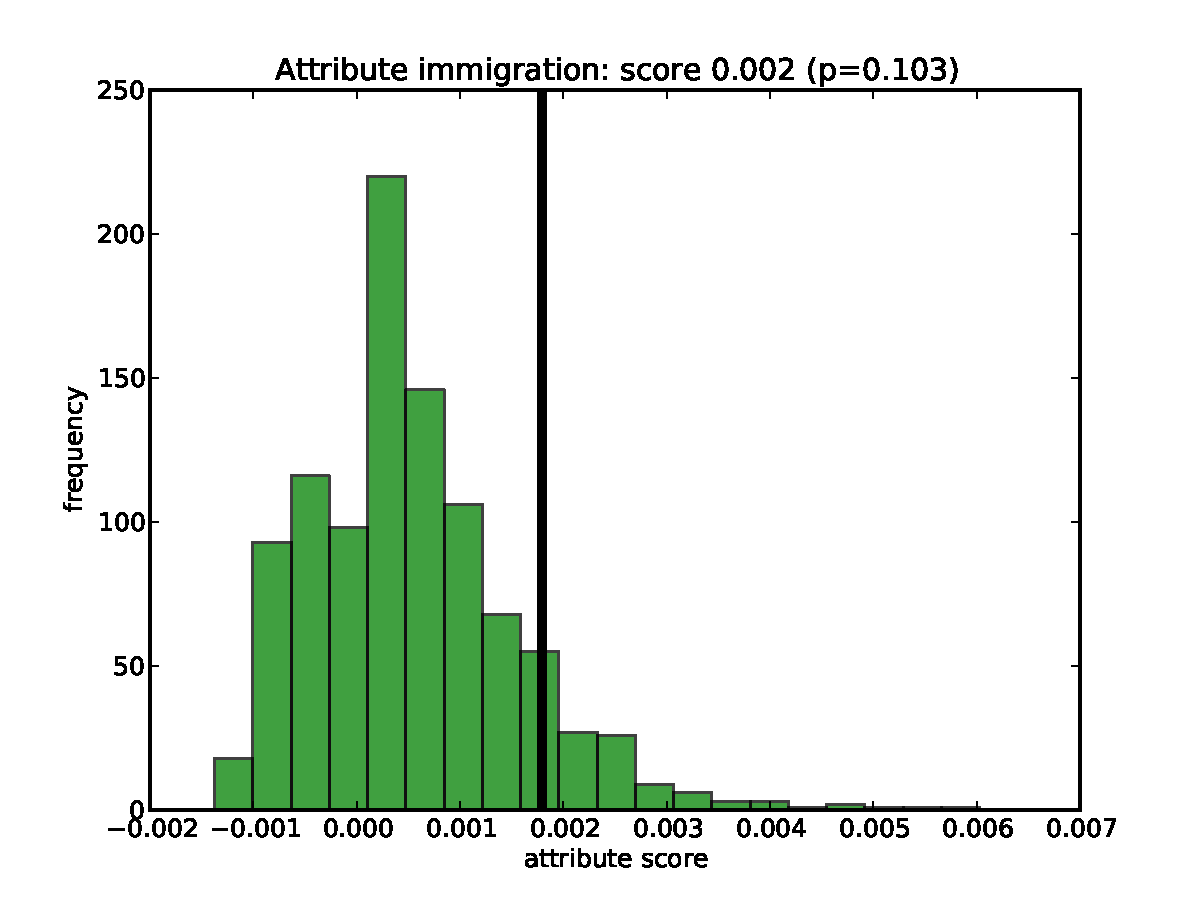
\includegraphics[width=8cm]{slike/att-score-null.pdf}
\caption{Rezultat permutacijske analize. Prikazana je porazdelitev informativnosti atributa, kot bi jo opazili, če bi bil razred primera naključen. Informativnost atributa na dejanskih, nenaključnih podatkih prikazuje vertikalna črta. Kar $10,3\%$ zmerjenih informativnost na naključnih podatkih je od te večja, zato tega atributa pri nadaljnji analizi ne bomo upoštevali.}
\label{f-att-score-null}
\end{center}
\end{figure}

Risanje grafov, kot je ta s slike~\ref{f-att-score-null}, je tipično zanimivo in informativno. Nikoli ne smemo zaupati samo golim številkam. Grafične ilustracije raznih analiz nam vedno pomagajo globlje razumeti problemsko domeno, čeprav vsi grafi niso ravno tisti, ki jih bomo vključili v naše končno poročilo. Da bo risanje takih grafov enostavneje, kodo za zgornji graf podajamo spodaj.

\begin{python}
import matplotlib.pyplot as plt

# plot score vs. null distribution for k-th worst attribute
k = 1
att, p = sorted(ps.items(), key=itemgetter(1), reverse=True)[k]
plt.close() # clear the drawing canvas
plt.hist(null[att], 20, facecolor="green", alpha=0.75)
plt.axvline(x=scores[att], color="k", linewidth=4)
plt.xlabel("attribute score")
plt.ylabel("frequency")
plt.title("Attribute %s: score %5.3f (p=%5.3f)" % (att.name, scores[att], p))
plt.savefig("att-score-null.pdf")
\end{python}

\section{Osnovni algoritmi za gradnjo modelov uvrščanja}

Razdelek bomo pričeli s pregledom danes morda najbolj uporabljanih tehnik uvrščanja v skupine. Razlogi za njihovo popularnost so različni. Naivni Bayesov klasifikator je preprost a mnogokrat presenetljivo natančen v napovedih. Prav tako preprost algoritem ima odkrivanje klasifikacijskih dreves, ki pa na realnih problemih tipično niso tako točna kot uvrščanje z naivnim Bayesom. Pristop s klasifikacijskimi drevesi je moč nadgraditi z uporabo t. im. gozdov, kjer namesto enega drevesa razvijemo več sto dreves. Z gozdom dreves napovedujemo tako, da njegova drevesa glasujejo. Tehnika podpornih vektorjev je na videz zelo drugačna od ostalih, a zaradi napovedne točnosti prav tako zelo popularna.

\subsection{Naivni Bayesov klasifikator}

Uvrščanje z naivnim Bayesovim klasifikatorjem uporablja Bayesovo pravilo za ocenjevanju verjetnosti. Na hitro ga izpeljimo. Opazujmo dva dogodka, $A$ in $B$ in $N$ opazovanj, pri katerih smo pojavitev dogodka $A$ zabeležili v $N_A$ primerih, pojavitev dogodka $B$ v $N_B$ primerih in pojavitev obeh dogodkov hkrati v $N_{AB}$ primerih. Velja $N=N_A+N_B-N_{AB}$. Verjetnost osnovnih dogodkov lahko ocenimo kot:
%
$$P(A)={N_A\over N}$$
$$P(B)={N_B\over N}$$
%
Podobno lahko ocenimo verjetnosti pogojnih dogodkov, kjer s $P(A|B)$ zapišemo verjetnost dogodka $A$ če vemo, da se je zgodil dogodek $B$:
%
$$ P(A|B)={N_{AB} \over N_{B}} $$
$$ P(B|A)={N_{AB} \over N_{A}} $$

Razmerje pogojnih verjetnosti zapisanih zgoraj je:
$${P(A|B) \over P(B|A)} = {N_{AB}\ N_A \over N_{B}\ N_{AB}} = {N_A/N \over N_B/N} = {P(A)\over P(B)}$$

Iz zgornjega sledi Bayesovo pravilo:
$$P(A|B)=P(A){P(B|A) \over P(B)}$$

Vzemimo primer $X$, ki je opisan z atributi $x_i$. Zanima nas verjetnost, da bo ta primer pripadal razredu $e$. To zapišemo kot pogojno verjetnost razreda pri danih vrednostih atributov, torej $P(e|X)$. Uporabimo Bayesovo pravilo:
%
$$ P(e|X) = P(e) {P(X|e) \over P(X)} $$
%
Predpostavimo tudi, da so atributi neodvisni glede na razred, in da lahko zapišemo verjetnost sestavljenega dogodka $P(X|e)$ kot produkt verjetnosti dogodkov $P(x_1|e)P(x_2|e)\ldots P(x_m|e)$. Ker verjetnosti pojavitve posameznega primera $P(X)$ iz podatkov ne moremo oceniti (zakaj? koliko primerov v primerjavi z velikostjo atributnega prostora bi potrebovali?), ocenimo raje razmerje verjetnosti razreda in vseh preostalih razredov (oz. verjetnosti dogodka in ne-dogodka):
%
$$ {P(e|X)\over P(\overline{e}|X)} = {P(e)\over P(\overline{e})} 
\prod {P(x_i|e)\over P(x_i|\overline{e})} $$

Ker je $P(e|X)+P(\overline(e)|X)=1$, lahko iz zgornjega razmerja izračunamo verjetnost $P(e|X)$. Vse člene na desni strani zgornje enačbe pa ocenimo iz podatkov.

V namene razlage odločitve je dobro zgornjo enačbo oziroma produkte, ki v njej nastopajo, pretvoriti v vsote. Seštevanje nam je tipično bližje kot množenje (koliko je 3.14 * 4.31? kolika pa je vsota teh števil?), in če moramo določeno odločitev obrazložiti, je vsekakor primernejše, če to storimo z vsoto prispevkov posameznih atributov kot pa s produktom. Tudi sicer si pri neformalnemu odločanju mnogokrat pomagamo s tem, da ``damo na vago'' dobre in slabe lastnosti variant, to je, razmišljamo o njihovem skupnem vplivu, ki ga dobivamo s seštevanjem prednosti in slabosti. Zato logaritmirajmo zgornjo enačbo:

$$ \log{P(e|X)\over P(\overline{e}|X)} = \log{P(e)\over P(\overline{e})} + \sum {P(x_i|e)\over P(x_i|\overline{e})} $$

Pri števni množici atributnih vrednosti, ki nastopajo v vsoti, vrednosti zgornjih členov tabeliramo, za izračun verjetnosti $P(e|X)$ iz izračunane vsote na desni strani zgornje pa izdelajmo tabelo preslikav. Celotno enačbo lahko za dan nabor podatkov predstavimo grafično v t.im. nomogramu (glej sliko~\ref{f-nomogram}).

\begin{figure}[htbp]
\begin{center}
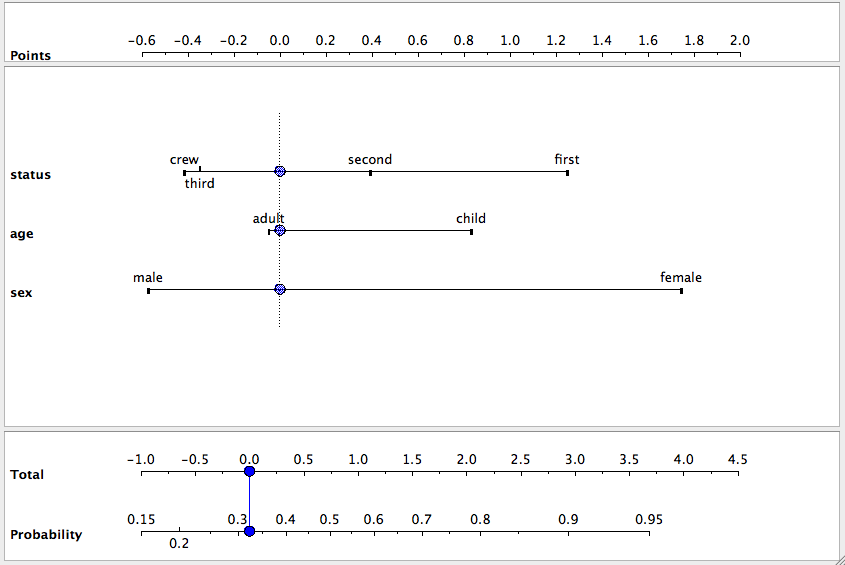
\includegraphics[width=11cm]{slike/nbc-titanic.png}
\caption{Naivni Bayesov nomogram, s katerim lahko ocenimo možnost preživetja na ladji Titanic pri danih potnikovih podatkih.}
\label{f-nomogram}
\end{center}
\end{figure}

\subsection{Klasifikacijska drevesa}

Klasifikacijska drevesa so ena najbolj osnovnih in enostavnih orodij za gradnjo napovednih modelov pri problemih z diskretnim razredom. Ker ste ta algoritem že dobro spoznali pri uvodnih predavanjih iz umetne inteligence, tu le na kratko. Osnovna ideja algoritma je razbitje začetne množice podatkov na čim bolj (razredno) čiste podmnožice. Za razbitje uporabimo en sam atribut, razbitje pa izvedemo na podlagi njegovih vrednosti. Tako smo na sliki~\ref{f-squares-triangles} za razbitje množice likov uporabili informacijo o njihovi barvi. Ker tipično podatki vsebujejo več atributov, izberemo tistega, ki vodi k najbolj čistim podmnožicam, to je tistega, katerega informativnost je za dano množico primerov največja. V osnovnem algoritmu postopek ponavljamo na dobljenih podmnožicah vse dokler te niso čiste, ali pa dokler nismo uporabili že vse atribute.

Rekurzivni algoritem zgradi drevo s korenom drevesa, v katerem smo imeli vse učne primere. Korenu sledijo vozlišča -- njegovi neposredni nasledniki, kjer smo primere iz osnovne množice razdelili skladno z vrednostmi najbolj informativnega atributa na podmnožice. Postopek smo ponovili vse do listov drevesa. Listom pripadajo primeri, ki izpolnjujejo pogoje oziroma imajo vrednosti atributov podane tako, kot je to zapisano na poti od lista do korena drevesa. Za vsak list lahko iz pripadajočih primerov ocenimo, kateri razred je najbolj pogost. Pravimo, da list uvršča v ta razred. Za potrebe uvrščanja se zato, glede na atributne vrednosti danega primera, sprehodimo od korena navzdol vse do lista, ki nam določa ustrezno uvrstitev.

Zgoraj smo opisali osnovni algoritem, tako imenovan algoritem ID3~\cite{} za gradnjo dreves. V izboljšanih verzijah algoritma pa lahko uporabimo tudi nekaj dodatnih trikov:
%
\begin{description}
\item[Obravnava zveznih atributov.] Te v danem vozlišču nadomestimo z binarnim atributom tako, da poiščemo mejo $t_X$, kjer skupina primerov razpade na skupino, kjer je $X<t_X$ in kjer je $X>=t_X$. Mejo $t_X$ izberemo tako, da vrednosti tega atributa, ki jih uporabljajo primeri, za katere iščemo razbitje, uredimo in preiščemo vse točke na sredini med dvemi zaporednimi vrednostmi. Izberemo tako mejno vrednost, kjer je informativnost (ocena) dobljenega binarnega atributa najvišja. Postopek imenujemo tudi kategorizacija oz. diskretizacija atributa, in je lahko primeren za predobdelavo celotne množice učnih primerov pri situacijah, kjer uporabljene metode ne znajo neposredno uporabiti zveznih atributov.

\item[Obravnava neznanih vrednosti atributov pri gradnji drevesa.] Te lahko preprosto zanemarimo oziroma jih ne upoštevamo pri ocenjevanju verjetnosti. Lahko pa jih upoštevamo tako, da ocenimo verjetnosti posameznih vrednosti in primere z neznanimi vrednostmi ustrezno ``razpršimo'' po podmnožicah.

\item[Neznane vrednosti atributov in uvrščanje.] Pri uvrščanju primerov, pri katerih nekateri atributi nimajo danih vrednosti (pravimo, da so te vrednosti neznane), lahko naletimo na vozlišče, ki zahteva poznavanje enega od teh atributov. Uvrstitev poiščemo tako, da se spustimo po vseh njegovih vejah in v vsaki poiščemo ustrezni razred, ki ga utežimo z verjetnostjo vrednosti atributa v danem vozlišču. Slednjo seveda dobimo pri učenju drevesa in si jo moramo v vozlišču, za namene uvrščanja, zapomniti.

\item[Rezanje dreves.] Drevesa tipično vodijo k drobljenju oziroma fragmentaciji problemske domene. Na razred namesto iz celotne množice primerov sklepamo iz veliko manjših podmnožic, ki pa s stališča statistike niso nujno ustrezne (bi bilo prav o pravičnosti igralne kocke razmišljati že po nekaj metih?). Bolje bi zato bilo zgraditi drevesa tako, da ta ne vodijo k premajhnim množicam v listih. Postopek se imenuje rezanje dreves. Lahko ga izvajamo vnaprej (na primer, postavimo mejo za najmanjše število primerov v listih), ali pa vzvratno tako, da zgradimo drevo in potem rekurzivno odstranjujemo nezanesljiva spodnja vozlišča. Eden od znanih postopkov za slednje imenujemo rezanje z zmanjševanjem napake \angl{minimal error prunning} in temelji na spremenjenem ocenjevanju verjetnosti tako, da pri njej upoštevamo še nekaj navideznih primerov, po enega iz vsakega razreda (t.im. ocena po Laplace-u~\cite{}) ali pa $m$ primerov, ki so porazdeljeni skladno z porazdelitvijo razredov v učni množici (t.im. $m$-ocena verjetnosti~\cite{}).

\item[Združevanje vrednosti atributov.] Nekateri diskretni atributi uporabljajo lahko (zelo) veliko število vrednosti in bi njihova uporaba pri gradnji dreves lahko vodila v takojšnjo veliko razpršitev primerov. Zato raje te vrednosti uredimo v podmnožice, ki jih poiščemo tako, da ima tako dobljeni atribut največjo informativnost. Zakaj za ocenjevanje slednje osnovna mera z informacijskim prispevkom ni primerna?
\end{description}

Tehnika gradnje in uporabe klasifikacijskih dreves ima vrsto prednosti. Je sorazmerno hitra, enostavna, zna obravnavati kakršnekoli podatke, ki jih lahko zapišemo v atributni obliki, deluje tudi na zelo velikih množicah podatkov. Uvrščanje je hitro. Model je odprt, ter ga je moč enostavno vizualizirati (slika~\ref{f-titanic-tree}) in ob njem razpravljati o možnih vzorcih v podatkih, ki jih je algoritem odkril.

\begin{figure}[htbp]
\begin{center}
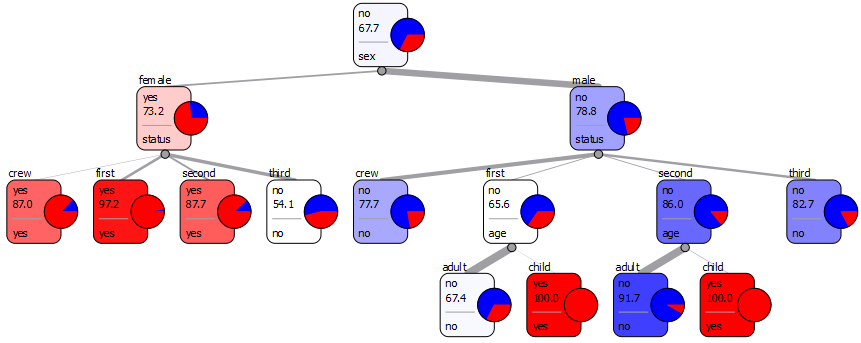
\includegraphics[width=15cm]{slike/titanic-tree.png}
\caption{Klasifikacijsko drevo zgrajeno iz podatkov o potnikih na ladji Titanic. Razred govori o preživetju nesreče. Debelina povezav med vozlišči drevesa ustreza številu primerov na teh povezavah. Barva vozlišč govori o verjetnosti prevladujočega razreda.}
\label{f-titanic-tree}
\end{center}
\end{figure}

Klasifikacijska drevesa pa imajo tudi pomanjkljivosti. O problemu fragmentacije, ki omejuje splošnost dreves in povzroči, da drevo sklepa o razredu na premajhnem vzorcu primerov, smo že govorili (kje? kdaj?). Tudi predstavljeni algoritem ne odkrije optimalnega drevesa, saj ne implementira vračanja in s tem kompleksnejše optimizacije. Drevesa so lahko izjemno velika in se lahko hitro preveč prilagodijo učnim podatkom. V splošnem drevo lahko modelira kompleksnejše povezave med primeri, na primer tudi take iz tabele~\ref{t-xor-boat}, a njih odkritje je pri uporabi univariatnih mer prepuščeno zgolj precej neverjetnemu naključju. Seveda pa lahko gradnjo dreves usmerjamo tudi s kontekstnimi merami kot je ReliefF, a s tem močno upočasnimo postopek gradnje.

Drevesa so prav tako občutljiva na lahko zelo majhne spremembe v učni množici. Prav lahko se zgodi, da sta dva ali več atributov med seboj zelo primerljiva po informacijski vsebini, in da majhne spremembe vplivajo na to, kateri atribut bomo izbrali. To situacijo lahko opazimo v korenu ali pa kakšnem drugem od notranjih vozlišč. V obeh primerih so lahko spremembe v strukturi drevesa izjemno velike, še posebej, če gre za vozlišče blizu vrha drevesa. Ta občutljivost je seveda nezaželena. Domenskim ekspertom bi želeli pokazati model, ki je stabilen, in se ne spreminja ob najmanjši spremembi učne množice. Izkorišča pa jo tehnika, o kateri govorimo spodaj.

\subsection{Naključni gozd}

Naključni gozd \angl{random forest} v uvrščanju sestavlja skupina klasifikacijskih dreves, ki pri klasifikaciji primera v razred glasuje~\cite{}. Naključni gozd napove razred, kamor primer uvršča večina klasifikacijskih dreves, ki gozd sestavlja. Najbolje bi bilo, da gozd sestavljajo drevesa, ki so med seboj različna in kjer vsak od dreves odkrije kakšen svoj, zanimiv koncept, ki se je skrival v podatkih. Podatke ti modeli osvetlijo iz različnih strani in potem skupaj o razredu glasuje. Več dreves več ve.

Taka drevesa dobimo v gozdu tako, da postopek malo ``ponaključimo''. In sicer:
\begin{enumerate}
\item Pričnemo z učno množico $D$, ki vsebuje $N$ primerov in $M$ atributov.
\item Izberemo število $m$, ki nam pove, med koliko naključno izbranih atributov iz primerov v vozliščih drevesa bomo izbrali najboljšega. Število $m$ naj bo veliko manjše od števila atributov, na primer $m=\sqrt{M}$. Izberemo tudi število dreves $K$ v gozdu, na primer $K=100$, ki ga želimo zgraditi. Nastavimo števec dreves, $i\leftarrow 1$.
\item Med $N$ primeri učne množice $D$ naključno z vračanjem izberemo novo množico primerov $D_i$ enake velikosti. To vrsto vzorčenja imenujemo metoda stremena \angl{bootstrap}. Seveda bodo v našem vzorcu posamezni primeri iz osnovne učne množice podvojeni.
\item Na množici primerov $D_i$ zgradimo klasifikacijsko drevo $T_i$, a tako, da v vsakem vozlišču naključno izberemo $m$ atributov, ki so uporabljeni v primerih vozlišča, in med njimi za delitev teh primerov izberemo najbolj informativnega upoštevaje razred primerov.
\item Če $i==K$ smo končali, sicer $i\leftarrow i+1$ in nazaj na korak 3.
\end{enumerate}

Tehnika naključnega gozda je danes ena od najbolj zanesljivih tehnik uvrščanja. Njene napovedne točnosti so tipično med najboljšimi. Tehnika podeduje vse prednosti klasifikacijskih dreves, zgubi pa možnost interpretacije modela, saj tega sedaj sestavlja vrsta modelov katerih vpliv na odločitve ni jasen in je odvisen od konteksta. Pristop v fazi gradnje modela ni med najhitrejšimi, ga pa je enostavno povzporediti.

Brieman~\cite{} je ob tem, ko je predlagal algoritem za gradnjo naključnega gozda, predlagal tudi metodo, ki oceni pomembnost, ki jo v gozdu imajo posamezni atributi pri pravilnem uvrščanju. Vsakemu vzorcu primerov $D_i$, na katerem smo zgradi drevo $T_i$,  določimo njegov komplement $D_i'=D-D_i$. Množica $D_i'$ je torej sestavljena iz primerov osnovne učne množice $D$, ki jih ni v vzorcu $D_i$ \angl{out-of-bag set}. Naj bo $C_i$ število primerov iz množice $D_i$, za katere je drevo $T_i$ pravilno napovedalo razred. Sedaj za vsak atribut $X$ premešajmo njegove vrednosti v $D_i$ in na taki, spremenjeni množici, izmerimo število pravilnih napovedi $C_{i,X}$. Pomembnost \angl{raw importance} atributa določimo kot:
%
$$ {\rm RI}(X)= {1\over K}\sum_{i=1}^K{C_i - C_{i,X}} $$

\subsection{Metoda podpornih vektorjev}

Metoda podpornih vektorjev je danes ena najbolj uporabljanih tehnik uvrščanja. Njeno osnovno varianto navadno izpeljemo za dvorazredne podatke, kjer je z linearno hiperravnino moč ločiti primere enega in drugega razreda (slika~\ref{f-svm}). Iščemo hiperravnino z največjim robom \angl{margin} do najbližjih primerov. Ti primeri ležijo na robu in jih imenujemo podporni vektorji. Razlog za to je, ker edino ti določajo lego hiperravnine, vse ostale primere pa bi lahko zanemarili. Razdalja katerekoli točke ${\bf x}$ do hiperavnine, ki jo določa normalni vektor ${\bf w}$ in njena razdalja do izhodišča $b$, je podana z enačbo $\mathbf{w}\cdot\mathbf{x} - b$. Če izberemo normalni vektor primerne dolžine, lahko za primere na robu zapišemo:
%
$$\mathbf{w}\cdot\mathbf{x} - b=\pm1$$
%
Zaradi enostavnosti zapišimo, da so razredi primerov $y_i$ označeni tako, da je $y_i=\pm 1$. Pri našem izbranem normalne vektorju, ki je usmerjen proti primerov z $y_i=1$, velja:
%
$$y_i(\mathbf{w}\cdot\mathbf{x_i} - b)\geq 1$$
%
Primeri so tako ali na robu ali pa od njega stran v smeri od hiperravnine. Naloga metode podpornih vektorjev je iskanje čim krajšega normalnega vektorja in konstante $b$ tako, da velja zgornja enačba.

\begin{figure}[htbp]
\begin{center}
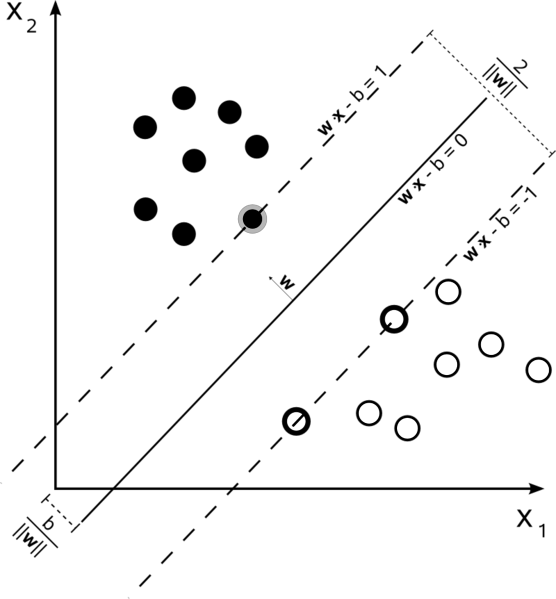
\includegraphics[width=8cm]{slike/svm.png}
\caption{Hiperravnina z največjim robom do primerov različnihrazredov. Primere na teh robovih imenujemo podporni vektorji.}
\label{f-svm}
\end{center}
\end{figure}

Matematični razvoj tehnike ni trivialen in presega okvir naših predavanj, vodi pa do elegantne rešitve, pri kateri rešujemo spodnji problem in iščemo koeficiente $\alpha_i$, ki so od 0 različni samo za podporne vektorje:
%
$$\min_{\mathbf{w},b } \max_{\bf{\alpha} } \left\{ \frac{1}{2}\|\mathbf{w}\|^2 - \sum_{i=1}^{n}{\alpha_i[y_i(\mathbf{w}\cdot \mathbf{x_i} - b)-1]} \right\}
$$
Izkaže se (to je, če pravilno matematično poiščemo rešitev), da je rešitev zgornjega problema v maksimizaciji izraza:
%
$$\tilde{L}(\mathbf{\alpha})=\sum_{i=1}^n \alpha_i - \frac{1}{2}\sum_{i, j} \alpha_i \alpha_j y_i y_j \mathbf{x}_i^T \mathbf{x}_j=\sum_{i=1}^n \alpha_i - \frac{1}{2}\sum_{i, j} \alpha_i \alpha_j y_i y_j k(\mathbf{x}_i, \mathbf{x}_j)$$
%
kjer so koeficienti $\alpha_i$ enak 0 za vse, razen za primere na robu. Funkcija $k$ je tako imenovana jedrna funkcija in je za naš primer linearne hiperravnine enaka
$k(\mathbf{x}_i,\mathbf{x}_j)=\mathbf{x}_i\cdot\mathbf{x}_j$. 

Čeprav na podlagi optimizacije in poiskanih primernih vrednosti $\alpha_i$ lahko izrazimo normalno hiperravnine, nas ta navadno celo več ne zanima, saj lahko uvrščanje zapišemo z enačbo:
%
$${\rm napoved}(x)={\rm sgn}(\sum_i \alpha_i y_i {\bf x_i}^T {\bf x}+b)$$

Matematična lepota zgoraj skicirane tehnike je, da jo je enostavno razširiti na probleme, kjer primeri različnih razredov niso popolno linearno ločljivi, in kjer meja ni več linearna oziroma kjer jedrna funkcija ni več skalarni produkt marveč kakšna bolj kompleksna funkcija.

\subsection{Najbližji sosedi}

Metoda $k$ najbližjih sosedov je sicer popularna, a zaradi tipično slabših napovednih točnosti služi bolj za primerjavo z drugimi metodami kot pa, da bi na osnovi nje gradili modele, ki bi bili sicer uporabni v praksi. Gre za leno metodo, ki si v fazi učenja samo zapomni vse učne primere, in celotno delo prenese na fazo uvrščanja. Uvršča tako, da za dani primer poišče $k$ njemu najbolj podobnih primerov (sosedov) upoštevaje vrednosti atributov in ne razreda, seveda. Napovedani razred je potem večinski razred teh najbližjih sosedov.

Izboljšane verzije tega algoritma ne upoštevajo vseh sosedov enako, ampak njihove razrede utežijo z mero podobnosti med primerov, ki ga želimo uvrstiti. Primeri iz učne množice, ki so bolj podobni novemu primeru, nosijo tako večjo težo.

\section{Ocenjevanje uspešnosti klasifikacijskih tehnik}

Ločujemo med merami uspešnosti klasifikacijskih tehnik in pristopi, kako te mere ocenimo. Pri slednjih je nadvse pomembno, da uspešnost nikoli ne ocenjujemo na učnih primerih. Ocenjevanje uspešnost mora biti izvedeno le na primerih, ki jih v postopku izdelave napovednega modela ali v kateremkoli njegovem delu nismo uporabili oziroma videli.

\subsection{Postopki ocenjevanja uspešnosti}

Iz osnovne, celotne množice z razredom označenih primerov $D$ izberimo vzorec učnih primerov $D_L$ in testnih primerov $D_T$, tako da, tipično, $D_L\cap D_T=\emptyset$ in $D_L\cup D_T=D$. Učne primere uporabimo za razvoj napovednega modela, katerega točnost nato preskusimo na testnih primerih. Da ocena točnosti ni odvisna od ene same delitve množice primerov, postopek večkrat ponovimo in poročamo o povprečni statistiki oziroma meri, ki smo jo uporabili za ocenjevanje algoritmov uvrščanja. Tehnike, ki jih pri tem lahko uporabimo, so:
\begin{description}
\item[Prečno preverjanje] reda $k$ \angl{k-fold cross validation}, kjer množico vseh primerov razdelimo na $k$ enakih množic in od teh pri vsakem od $k$ korakov eno uporabimo za testiranje, vse ostale pa za učenje.
\item[Izloči enega] \angl{leave-one-out}, pri čemer iz množice primerov vsakič izločimo en sam primer, na katerem bomo zgrajeni napovedni model testirali, vse ostale primere pa uporabimo za gradnjo modela. Postopek je predvsem primeren za manjše nabore podatkov.
\item[Metoda stremena] \angl{bootstrap} kjer iz množice z $N$ primeri z vračanjem naključno izberemo enako veliko množico za učenje in vse neizbrane primere uporabimo za testiranje. Vzorčenje, gradnjo modela in testiranje večkrat ponovimo. Tipično je takih ponovitev sto ali nekaj sto, tudi do tisoč.
\end{description}

\subsection{Mere}

\begin{table}[htbp]
\caption{Kontingenčna tabela ali tabela napak \angl{confusion matrix}.}
\label{t-confusion-matrix}
\begin{center}
\begin{tabular}{rcccc}
& & \multicolumn{2}{c}{Dejanska vrednost} \\ 
& & $+$ & $-$ \\
\cmidrule(r){3-4}
Napovedana & $+$ & True Positive ($TP$) & False Positive ($FP$) & $P'$ \\
vrednost & $-$ & False Negative ($FN$) & True Negative ($TN$) & $N'$ \\ \cmidrule(r){3-4}
& & $P$ & $N$ \\
\end{tabular}
\end{center}
\end{table}

\begin{description}
\item[zadetek] (TP), \angl{true positive}
\item[pravilna zavrnitev](TN), \angl{true negative}
\item[napačno pozitiven, lažni alarm] (FP), napaka I. reda \angl{false positive}
\item[pogrešek] (FN), napaka II. reda \angl{false negative}
\item[občutljivost, priklic] \angl{sensitivity, true positive rate, recall}, $TPR = {TP / P} = {TP / (TP+FN)} $
\item[delež napačno pozitivnih], odpadek (FPR), \angl{false positive rate, fall-out} $FPR = FP / N = FP / (FP + TN)$
\item[točnost] (ACC), \angl{accuracy}, $ACC = (TP + TN) / (P + N)$
\item[specifičnost], stopnja pravilne zavrnitve (SPC), \angl{specificity, true negative rate}, $SPC = TN / N = TN / (FP + TN) = 1 - FPR$
\item[natančnost], delež pravilnih pozitivnih (PPV), \angl{positive predictive value, precision} $PPV = TP / (TP + FP)$
\item[delež pravilnih negativnih] (NPV), \angl{negative predictive value}, $NPV = TN / (TN + FN)$
\item[mera F1] (F1) \angl{F1 score}, $F1 = 2TP^2/(P+P')$
\end{description}

\subsection{Površina pod krivuljo ROC}

Prav posebna mera je površina pod krivuljo ROC \angl{area under Receiving Operator Characteristics curve} in zato zasluži poseben razdelek. Mero so najprej uporabili v ameriški vojski tekom druge svetovne vojne in z njo skušali oceniti radariste ter njihovo točnost pri razlikovanju med zavezniškimi in agresorjevimi letali na radarskem zaslonu. Ocenjevali so jih v različnih pogojih (dopoldne, zvečer, po neprespani noči, ...) in ob različnih časih ter skušali, ne glede na njihovo stanje, radariste kar najbolj objektivno rangirati, od teh zelo uspešnih do drugih, ki so bolj često delali napake. Mero so ponovno odkrili v 1970-ih in jo najprej uporabljali v radiologiji, kasneje pa na celotnem področju medicine. Da bi jo potem znova odkrili na prelomu stoletja in pričeli množično uporabljati na celotnem področju statistike in odkrivanja znanj iz podatkov.

Oglejmo si najprej konstrukcijo krivulje ROC na primeru. Denimo, da smo že zgradili model uvrščanja in bi radi ocenili njegovo točnost na testnih primerih. Naš klasifikacijski problem je dvovrednostni, napovedni model pa zna napovedati verjetnosti ciljnega razreda $p(+|X)$, kjer je $X$ atributno opisan primer.

\begin{table}[htbp]
\caption{Testni primeri z dejanskim razredom in verjetnostjo razred ``yes'', kot jo je predlagal napovedni model, katerega točnost ocenjujemo. Primeri so urejeni skladno z napovedano verjetnostjo.}
\label{t-auc}
\begin{center}
\begin{tabular}{cc}
\toprule
Razred & $p(+|X)$ \\
\midrule
+ & 0.89 \\
+ & 0.80 \\
+ & 0.80 \\
- & 0.80 \\
+ & 0.63 \\
- & 0.33 \\
+ & 0.33 \\
- & 0.10 \\
- & 0.10 \\
- & 0.10 \\
\bottomrule
\end{tabular}
\end{center}
\end{table}

Točnost uvrščanja primerov s tabele~\ref{t-auc} je odvisna od praga verjetnosti $p_T$, nad katerimi bomo razglasili, da primeri pripadajo pozitivnemu razredu. Pri tem bomo opazovali $TPR$, to je delež pravilno napovedanih pozitivnih primerov med vsemi dejansko pozitivnimi \angl{true positive rate}, in $FPR$, delež negativnih primerov, za katere je bila napoved napačna \angl{false positive rate}. Izrazimo ti dve meri še z notacijo iz prejšnjega razdelka:
$$ TPR = {TP \over P} $$
$$ FPR = {FP \over N} $$

Vzemimo, da vse primere razglasimo kot pozitivne ($p_T<0.10$). Na ta način smo pravilno ``ulovili'' vse dejansko pozitivne primere in s tem dosegli najvišji delež pravilno napovedanih pozitivnih primerov med vsemi dejansko pozitivni primeri ($TP=P$, $TPR=1.0$). Tudi $FPR$ je s tem maksimalni, 1.0, saj smo vse negativne primere napačno uvrstili med pozitivne.

Drugače pa je, če vse primere iz testne razglasimo kot negativne ($p_T>0.89$). Primerov, ki bi jih razglasili za pozitivne, ni, zato $TPR=0$ in $FPR=0$.

Vse ostale vrednosti $TPR$ in $FPR$ bodo, za prag, ki ga izberemo med zgornjima dvema skrajnima mejama, nekje med 0 in 1. Najbolj zaželen prag bi bil tam, kjer bi vse razvrstitve v pozitivni razred bile pravilne in nobena ne bi bila nepravilna. V tej točki bi bil $TPR=1$ in $FPR=0$. Ali za naš primer taka vrednost praga obstaja?

Preskusimo sedaj vse možne mejne vrednosti $p_T$, kjer bi se nam vrednosti $TPR$ in $FPR$ lahko spremenile. Za naše podatke imamo štiri intervale, kjer lahko poiščemo take meje. Med 0.89 in 0.80, med 0.80 in 0.63, med 0.63 in 0.33, in med 0.33 in 0.10. Kje v teh intervalih bo dejansko naša mejna vrednost ni pomembno. Za te štiri meje izračunajmo sedaj vrednosti $TPR$ in $FPR$ in te vnesimo v graf (slika~\ref{f-roc}).

\begin{figure}[htbp]
\begin{center}
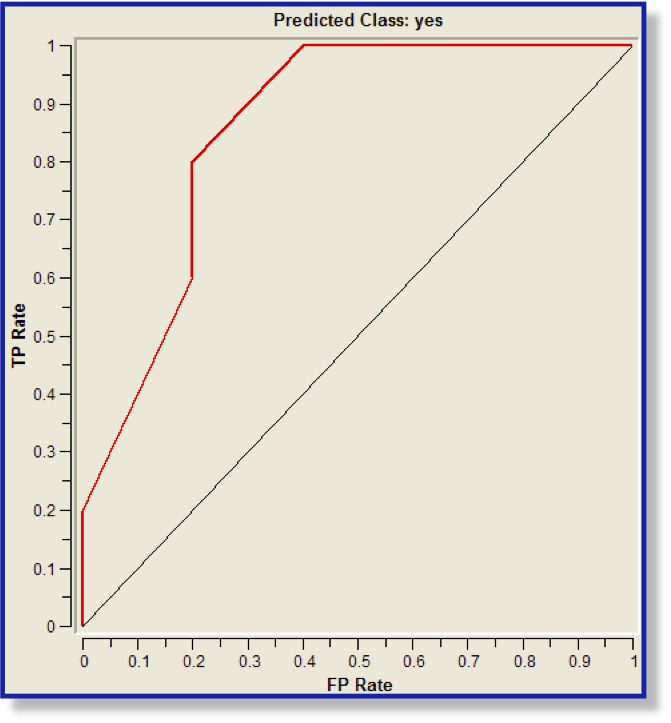
\includegraphics[width=7cm]{slike/roc.png}
\caption{Krivulja ROC za podatke s tabele~\ref{t-auc}.}
\label{f-roc}
\end{center}
\end{figure}

Obstaja tudi hitrejši način izrisa krivulja $ROC$, ki zahteva ureditev primerov po napovedani verjetnosti ciljnega razreda (kot smo to storili v tabeli~\ref{t-auc}). Postopek je naslednji:
%
\begin{enumerate}
\item Izrišemo graf z mrežo $1/N$ horizontalno in $1/P$ vertikalno.
\item Uredimo primere v seznam $L$ po padajoči verjetnosti napovedi v ciljni razred.
\item Pričnimo v točki (0,0).
\item Izberimo in iz seznama $L$ izključimo primere z najvišjo napovedano verjetnostjo. Naj ti primeri vključujejo $n_+$ primerov iz pozitivnega razreda, in $n_-$ primerov iz negativnega razreda. V mreži grafa se premaknimo $n_+$ razdelkov desno in $n_-$ razdelkov navzgor.
\item Če $L$ ni prazen, skoči na korak 4, sicer končaj.
\end{enumerate}

\begin{figure}[htbp]
\begin{center}
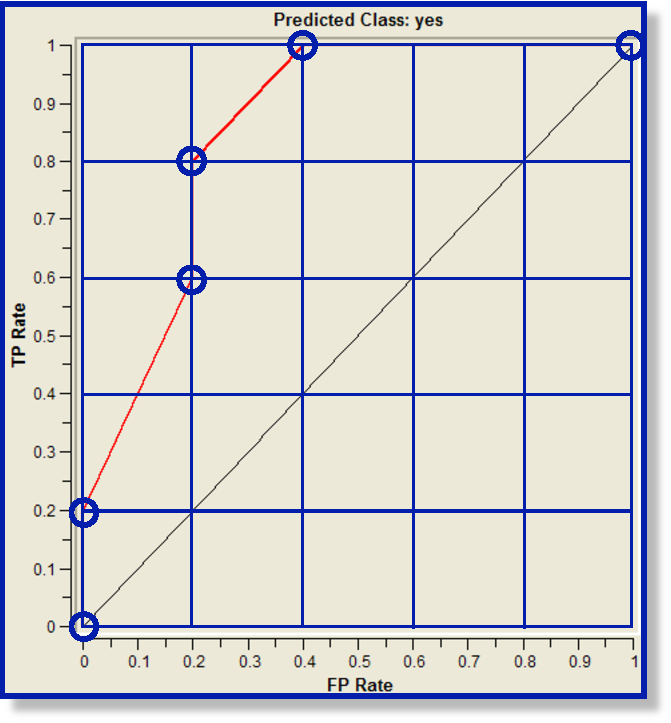
\includegraphics[width=7cm]{slike/roc-walk.pdf}
\caption{Mreža za izris krivulje ROC in sprehod po njenih točkah skladno s primeri s tabele~\ref{t-auc}.}
\label{f-roc-walk}
\end{center}
\end{figure}

Opazimo, da zgoraj opisan algoritem pravilno razpozna obe meri $TPR$ in $FPR$ za vse možne vrednosti praga verjetnosti (slika~\ref{f-roc-walk}).

Površino pod krivuljo ROC označimo z $AUC$. Pri naključnih napovedih pričakujemo, da bodo v obhodu zgornjega algoritma šli približno po diagonali grafi in bo $AUC=0.5$. To je tudi spodnja meja za to mero in je karakteristična za neuspešen napovedni model. Dejansko je meja za uspešne modele tipično pri $AUC=0.75$, modeli, ki imajo visoko napovedno točnost, pa imajo $AUC$ nekje nad $0.9$.

Površina pod ROC krivuljo pa ima še eno zanimivo lastnost. Če opazujemo sprehod po mreži za izris ROC krivulje, opazimo, da površina pod vsakem segmentom ravno ustreza številu napačno razvrščenih primerov, katerih verjetnost pozitivnega razreda je nad določeno mejo. $AUC$ ustreza verjetnosti, da za naključno izbrani primer $X^+$ iz pozitivnega razreda in naključno izbrani primer $X^-$ iz negativnega razreda velja $p(+,X^+) > p(+, X^-)$.

\section{Izbor atributov}

V praksi se lahko srečamo s problemskimi domenami, kjer so podatki opisani z veliko množico atributov. Na primer, nekaj sto ali več tisoč, včasih tudi več sto tisoč atributov. Pričakujemo lahko, da so nekateri med temi atributi zares pomembni in nosijo informacijo o razredu, nekateri pa so nepomembni in samo otežujejo oblikovanje napovednega modela ali pa celo preprečijo, da bi gradnja modela bila uspešno, to je, da bi zgradili model z dobro napovedno točnostjo. Uvrščanje s tehniko najbližjih sosedov je primer metode, kjer lahko velika množica neinformativnih atributov zelo škoduje. Prijemi izbora atributov imajo za cilj zmanjšanje atributnega prostora in posledično, upajmo, izboljšanje točnosti modela, ki se ga iz tako spremenjenih primerov naučimo.

V grobem ločimo dve družini pristopov k izboru atributov. Pri prvi, kjer najdemo pristope s filtriranjem atributov \angl{filter approach}, uporabimo izbrano mero za ocenjevanje atributov in na podlagi te izberemo najboljše med atributi. Pri izboru nam lahko zelo pomaga perturbacijski test (glej razdelek~\ref{c-attribute-scoring}), kjer lahko sprejmemo na primer vse atribute z značilnim odstopanjem od ničelne porazdelitve (na primer izberemo $\alpha=0.01$).

Druga družina pristopov, imenovana pristopi z ovojnico \angl{wrapper approaches}, pa izbira atribute skladno z uspešnostjo izbrane tehnike razvrščanja. Točnost te tehnike ${\rm Acc}$, ki jo za določeno mero točnosti na primer ocenimo s prečnim preverjanjem, je odvisna od množice izbranih atributov $X'\in\mathcal{X}$, ${\rm Acc}={\rm Acc}(\mathcal{X}')$. Med atributi izberi podmnožico, pri kateri je tako ocenjena točnost dane tehnike uvrščanja najvišja:
%
$$ {\mathcal X}^* = \argmax_{{\mathcal X}'\subset{\mathcal X}}{\rm Acc}(\mathcal{X}') $$
%
Seveda vseh možnih podmnožic atributov ne moremo preiskati. Tehnike z ovojnico zato uporabljajo različne hevristične prijeme. Na primer, pričnejo z najbolj informativnim atributom in tej množici dodajo po en atribut tako, da se z njim točnost uvrščanja najbolj poveča. Postopek prekinemo, kot točnost pade. Podobno lahko pričnemo z vsemi atributi in iz te množice postopno odvzemamo atribute. Ali pa za bolj izčrpno preiskovanje prostora množic atributov uporabimo genetske algoritme.

\section{Izbor metode uvrščanja in njenih parametrov}

Klasična napaka: na celotni učni množici s prečnim preverjanjem ocenimo, pri kateri vrednosti njenih parametrov (npr. $k$ kot število najbolj podobnih primerov, ki jih opazujemo pri tehniki najbližjih sosedov) daje izbrana metoda najboljše rezultate. Potem poročam o na ta način izračunani meri točnosti.

Kaj je tu narobe? Za določanje parametrov metode smo uporabili celotno učno množico in potem na tej isti množici poročali o uspešnosti tega postopka. Izbor optimalnih parametrov metode je, ravno tako kot gradnja modela, del razvoja napovednega modela, ki ga je potrebno preveriti na neodvisni testni množici. Tega nismo storili, rezultati, o katerih smo poročali, pa so lahko izrazito prilagojeni podatkov, na katerih smo parametre optimizirali.

Kako bi uspešnost izbora parametrov pravilno ocenili? S prečnim preverjanjem, kjer pa bi vrednosti parametra najprej ocenili znotraj vsake množice učnih primerov z dodatnim, t.im. notranjim prečnim preverjanjem. Ko bi na ta način metodi določili vrednost njenih parametrov, bi potem njeno točnost s temi parametri ocenili na testnih primerih. Ker bi v zunanji zanki prečnega preverjanja postopek ponovili npr. desetkrat, bi na ta način dobili deset različnih vrednosti za parametre metode. Lahko bi nato poročali o povprečni vrednosti teh parametrov in priporočili, da se ti uporabljajo pri učenju na podatkih iz izbrane problemske domene.

Podobno kot s parametri učenja je z izborom najboljše tehnike gradnje napovednih modelov. Tudi tu med množico dostopnih tehnik izberemo eno na podlagi notranjega prečnega preverjanja. Pri 10-kratnem zunanjem prečnem preverjanju se nam seveda lahko zgodi, da smo na ta način izbirali druge tehnike gradnje modelov uvrščanja. A to ni problematično, saj smo ravno želeli oceniti naš celotni postopek, to je izbor prave metode predobdelave podatkov, učenja in z njo gradnjo napovednega modela.
